\section{Matyas Function}
\label{sec:app:test:matyas}
  The \emph{Matyas function}, known for its simplicity and convex nature, is a 
  standard test problem in the field of optimization algorithms.
  Despite its apparent simplicity, it provides invaluable insights into an
  algorithm's performance and behavior.

  \begin{definition}[Matyas Function]
    \label{def:app:test:matyas}
    The \emph{Matyas function}, denoted as \(f: \mathbb{R}^2 \rightarrow 
    \mathbb{R}\), is formulated as:

    \begin{equation}
      \label{eq:app:test:matyas}
      f(x,\, y) = 0.26(x^2 + y^2) - 0.48xy
    \end{equation}
    
    where:
    
    \begin{itemize}
      \item \(x,\, y \in \mathbb{R}\) denote the decision variables.
    \end{itemize}
  \end{definition}

  The Matyas function reaches its global minimum at the origin, with \(f(0, 0) =
  0\).
  The contour and surface visualizations of the Matyas function, offering
  perspectives on its topographical attributes, are presented in 
  \vref{fig:app:test:matyas}.

  \begin{figure}[ht!]
    \centering
    \begin{subfigure}[b]{0.45\textwidth}
      \centering
      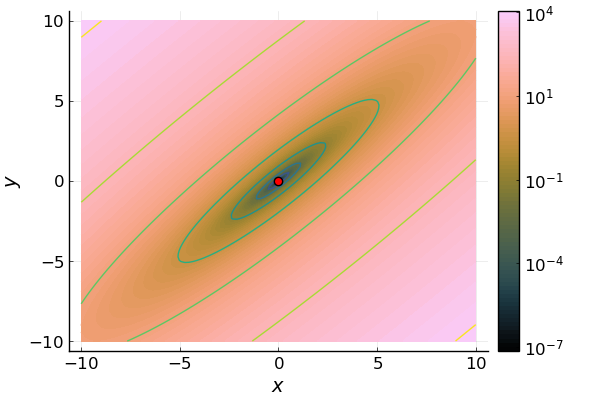
\includegraphics[width=\textwidth]{img/test_functions/matyas_contour.png}
      \caption{
        Contour plot of the Matyas function with a red dot indicating the global
        minimum
      }
      \label{fig:app:test:matyas:contour}
    \end{subfigure}
    \hfill
    \begin{subfigure}[b]{0.45\textwidth}
      \centering
      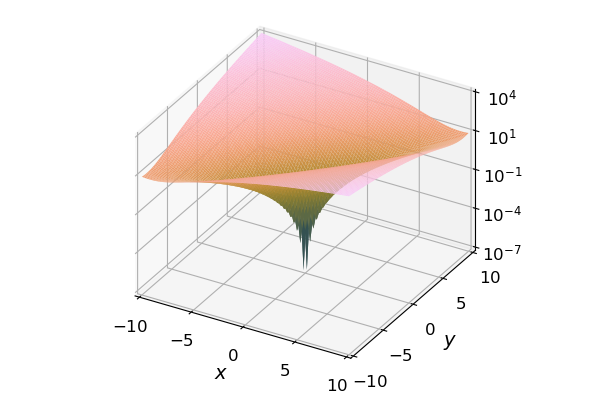
\includegraphics[width=\textwidth]{img/test_functions/matyas_surface.png}
      \caption{Surface plot of the Matyas function}
      \label{fig:app:test:matyas:surface}
    \end{subfigure}
    \caption{Contour and Surface Visualizations of the Matyas Function}
    \label{fig:app:test:matyas}
  \end{figure}
